%% March 2018
%%%%%%%%%%%%%%%%%%%%%%%%%%%%%%%%%%%%%%%%%%%%%%%%%%%%%%%%%%%%%%%%%%%%%%%%%%%%
% AGUJournalTemplate.tex: this template file is for articles formatted with 
% LaTeX
%
% This file includes commands and instructions
% given in the order necessary to produce a final output that will
% satisfy AGU requirements, including customized APA reference formatting.
%
% You may copy this file and give it your
% article name, and enter your text.
%
%%%%%%%%%%%%%%%%%%%%%%%%%%%%%%%%%%%%%%%%%%%%%%%%%%%%%%%%%%%%%%%%%%%%%%%%%%%%
% PLEASE DO NOT USE YOUR OWN MACROS
% DO NOT USE \newcommand, \renewcommand, or \def, etc.
%
% FOR FIGURES, DO NOT USE \psfrag or \subfigure.
% DO NOT USE \psfrag or \subfigure commands.
%%%%%%%%%%%%%%%%%%%%%%%%%%%%%%%%%%%%%%%%%%%%%%%%%%%%%%%%%%%%%%%%%%%%%%%%%%%%
%
% Step 1: Set the \documentclass
%
% There are two options for article format:
%
% PLEASE USE THE DRAFT OPTION TO SUBMIT YOUR PAPERS.
% The draft option produces double spaced output.

%% To submit your paper:
\documentclass[draft,linenumbers]{agujournal2018}
\usepackage{apacite}
\usepackage{graphicx}
\usepackage[demo]{rotating}
% \usepackage{url}    %this package should fix any errors with URLs in refs.
\draftfalse 		% This option makes double space

%%%%%%%
% \usepackage{trackchanges}
% uncomment the line above to use the TrackChanges package to mark revisions 
% if needed.
% The trackchanges package adds five new LaTeX commands:
%
%  \note[editor]{The note}
%  \annote[editor]{Text to annotate}{The note}
%  \add[editor]{Text to add}
%  \remove[editor]{Text to remove}
%  \change[editor]{Text to remove}{Text to add}
%
% complete documentation is here: http://trackchanges.sourceforge.net/
%%%%%%%


% Now, type in the journal name: \journalname{<Journal Name>}

% ie, \journalname{Journal of Geophysical Research}
%% Choose from this list of Journals:
%
% JGR-Atmospheres
% JGR-Biogeosciences
% JGR-Earth Surface
% JGR-Oceans
% JGR-Planets
% JGR-Solid Earth
% JGR-Space Physics
% Global Biochemical Cycles
% Geophysical Research Letters
% Paleoceanography
% Radio Science
% Reviews of Geophysics
% Tectonics
% Space Weather
% Water Resource Research
% Geochemistry, Geophysics, Geosystems
% Journal of Advances in Modeling Earth Systems (JAMES)
% Earth's Future
% Earth and Space Science
% Geohealth
%

\journalname{Water Resource Research}

\begin{document}

%% ------------------------------------------------------------------------ %%
%  Title
% (A title should be specific, informative, and brief. Use
% abbreviations only if they are defined in the abstract. Titles that
% start with general keywords then specific terms are optimized in
% searches)
%% ------------------------------------------------------------------------ %%

% OPTION 1 - Antonio Preziosi
\title{Fine Sediment Deposition and Filtration Under Losing and Gaining Conditions: A Particle-Tracking 
Model Approach}

% OPTION 2 - Antonio Preziosi
% \title{Particle tracking model for kaolinite deposition in flumes under 
% losing or gaining flow conditions}

% OPTION 3 - Antonio Preziosi
% \title{Colloid exchange between a gaining/losing stream and streambed: 
% A particle tracking approach}

% Example: \title{This is a test title}

%% ------------------------------------------------------------------------ %%
%  AUTHORS AND AFFILIATIONS
%% ------------------------------------------------------------------------ %%

% Authors are individuals who have significantly contributed to the
% research and preparation of the article. Group authors are allowed, if
% each author in the group is separately identified in an appendix.)

% List authors by first name or initial followed by last name and
% separated by commas. Use \affil{} to number affiliations, and
% \thanks{} for author notes.
% Additional author notes should be indicated with \thanks{} (for
% example, for current addresses).

% Autores del paper
\authors{Antonio Preziosi-Ribero\affil{1}\thanks{Ciudad Universitaria,
Bogot\'{a}, Colombia}, Aaron I. Packman\affil{2}, Jorge A. Escobar-Vargas\affil{1, 3}, Colin B. Philips\affil{2}, Leonardo David Donado\affil{1}, and Shai Arnon\affil{4}}

% Afiliaciones de los autores
\affiliation{1}{Universidad Nacional de Colombia, Facultad de Ingenier\'{i}a,
Bogot\'{a}, Colombia}
\affiliation{2}{Department of Civil and Environmental Engineering, 
Northwestern University, Evanston, IL, USA}
\affiliation{3}{Departamento de Ingenier\'{i}a Civil, Pontificia Universidad
Javeriana, Bogot\'{a}, Colombia}
\affiliation{4}{Zuckerberg Institute for Water Research, the J. Blaustein Institutes for Deseart Research, Ben-Gurion University of the Negev, Beersheba, Israel}

% \affiliation{4}{Fourth Affiliation}

% \affiliation{=number=}{=Affiliation Address=}
%(repeat as many times as is necessary)

%% Corresponding Author:
% Corresponding author mailing address and e-mail address:

% (include name and email addresses of the corresponding author.  More
% than one corresponding author is allowed in this LaTeX file and for
% publication; but only one corresponding author is allowed in our
% editorial system.)

% Example: \correspondingauthor{First and Last Name}{email@address.edu}

\correspondingauthor{Antonio Preziosi-Ribero}{apreziosir@unal.edu.co}

%% Keypoints, final entry on title page.

\begin{keypoints}
\item We developed a Particle-Tracking model for fine sediments' deposition taking into account gaining and losing groundwater into the stream
\item Patterns of clay deposition depend on the velocity profile generated by the free surface flow conditions and groundwater vertical flow
\item Fine particle deposition is controlled by gaining or losing groundwater along with the ins-stream processes
\end{keypoints}

% ============================================================================
% ABSTRACT
% ============================================================================

\begin{abstract}
Fine particle deposition in rivers plays a major role in riverine ecology and biogeochemistry by altering hyporheic exchange rates. Moreover, it is ubiquitous within streams and rivers across all flow stages. However, fine particle deposition remains poorly understood in river hydrodynamics and continuum model treatments like the Advection Dispersion Equation require modifications to represent the process accurately. To enhance understanding of fine particle dynamics, we developed a numerical Particle-Tracking model that simulates deposition within an idealized sand bedform under losing, neutral and gaining groundwater flow conditions. This model takes into account the velocity profiles generated by free surface and groundwater flow and incorporates a stochastic function that simulates filtration within the sand bed. Our simulated results qualitatively agree with previous laboratory flume experimental results of clay particle deposition. Our results suggest that fine particle deposition patterns and residence time functions depend heavily on the imposed groundwater flow conditions and bed filtration properties. The spatial pattern of particle deposition is a direct result of porewater velocity profiles, while the concentration depends on filtration dynamics within the bed. These findings indicate that the deposition of fine particles could be substantially altered by bed heterogeneity and transient effects that alter bed permeability and pore water velocity profiles and flow patterns.
\end{abstract}

% ============================================================================
% INTRODUCTION SECTION - NOT CORRECTED FROM PACKMAN'S COMMENTS YET... 02/12 WILL BE DONE
% ============================================================================
\section{Introduction} \label{Introduction}

% 1. GENERALITIES ON SEDIMENT DEPOSITION AND A BRIEF CONCEPT OF WHAT IS CONSIDERED AND HOW DOES IT WORK IN RIVERS (PARTINGTON)
Rivers as integrators of their catchments represent collections of different geological, biological, chemical and ecological processes. Many of these phenomena depend on the exchange of momentum, matter and energy between the river and the surrounding groundwater systems, i.e. Hyporheic Exchange (HE) \citep{Boano2014}. This exchange is present throughout the river and can occur across a range of different scales with varying magnitudes \citep{Buendia2014}. Nevertheless, HE is a phenomenon that is affected by fine particle transport and deposition within the stream because of filtering processes present in the river bed that can lead to clogging and siltation \citep{Crenshaw2002,Mendoza2017}. This interaction between sediment transport and deposition can alter nutrient fluxes in rivers and plays an important role in determining the quality of the aquatic ecosystem as a whole \citep{Partington2017}. Indeed, contaminant transport and carbon and nutrient dynamics are closely related to HE and sediment deposition \citep{Hope1994,Gottselig2014}.

Sediment deposition, ubiquitous within rivers, is driven by the interactions of river flow and bed surface topography \citep{Packman2000,Packman2000b,Harvey2012}. Fine sediments are typically defined as minerals or aggregations of organic compounds with sizes smaller than $10 \ \mu m$ \citep{Harvey2012,Drummond2014,Drummond2018}. Among sediments, fine particles can serve dual roles as both nutrients and contaminants and due to their small size are easily suspendable, thus they can travel freely travel within streams and rivers even at low flow. However, fine particles may deposit through interactions with geomorphic features such as dunes, pools, riffles, and bars which induce hyporheic flow \citep{Buendia2014}. Moreover, they are well known to deposit in the stream bed and resuspend into the free flow with some periodicity \citep{Drummond2015} depending on the surface flow driven by extreme events like storms \citep{Drummond2017}. However, their retention in the stream bed is known to affect hyporheic flow, the exchange of nutrients, and alter physical properties of the media like porosity and permeability \citep{Crenshaw2002,Mendoza2017}.

Along with sediment transport, fine particle deposition has recently been fostered by land use changes \citep{Gartner2012,Wohl2015}, and both have effects on the biogeochemical processes as nutrient and carbon cycling \citep{Hope1994,Gottselig2014}, since these particles clog the river bed in different spots \citep{Brunke1999}. Indeed, fine particle deposition and transport has effects on the growth of microbial communities and favors denitrification processes due to the lack of oxygen in clogged zones \citep{Navel2011}. Thus, the understanding of fine particle dynamics in riverbeds is a challenge for river restoration and management. The scope of the present work is to understand physically the link between the different processes that control sediment deposition based on previous findings and models. 

% 3. THE ROAD SO FAR... 
In part due to the complexity of natural rivers, laboratory experiments have represented one of the primary tools for understanding the coupling between HE and sediment deposition \citep{Elliott1997b,Marion2002,Salehin2004a}. An important insight gained from early experimental efforts suggests that fine particle deposition occurs not only by gravitational deposition \citep{Vanoni1974}, but that there are other key physical parameters that control the phenomenon invalidating classical assumptions of exclusive gravitational settling of fine particles. Flume models necessarily represent particle deposition at a local scale and due to considerable variability within these systems it can remain challenging to isolate specific mechanisms and processes in the coupling of HE and sediment deposition. Understanding the role of regional groundwater patterns that result in losing and gaining flow on fine sediment deposition has only been evaluated in a handful of experiments \citep{Fox2014,Fox2018}. 

At the reach scale the exchange between surface flows and groundwater has been heavily recorded and modeled  \citep{Woessner2000a,Cardenas2004,Harvey2012}. The results of these experiments suggest that the river bed acts as a filter that traps all kind of fine particles with different mechanisms (i.e., filtration, clogging and straining). Another relevant result from these experiments is the fact that particle deposition changes the physical properties of the river beds, like porosity and permeability. However, reach-scale models are not able to accurately quantify the effects of groundwater flow on sediment deposition patterns at small scales. Thus, it is necessary to explore further this aspect to validate how the interaction between free surface flow and groundwater flow hinders or fosters sediment deposition in streams. 

Regarding the numerical models, particle deposition has been assessed under the assumptions of the advective pumping model, that generates flow paths in the stream bed due to the change of pressure generated by the presence of ripples and dunes \citep{Elliott1997,Elliott1997b}. Some of these models have mainly focused on estimating hydrodynamic fields and solute transport using the continuum mechanics expressions like the Advection Dispersion Equation (ADE) \citep{Cardenas2006,Cardenas2007f,Cardenas2007b,Boano2007b,BayaniCardenas2008c,Trauth2013}. Instead, models that use numerical particles that represent fine sediments have been used to assess deposition patterns \citep{Packman2000}, using known velocity profiles in local scales. The Particle Tracking (PT) approach can also be used at reach scales to model nutrient uptake in rivers \citep{Li2017}. Advantages of using PT models are that this technique is useful for a long range of scales \citep{Delay2005}, and that physical and chemical processes can be split and analyzed separately. However, modeling the physical process of particle deposition under different groundwater flow conditions remains a major challenge for river hydrodynamics, since current models do not include explicit terms that account for vertical groundwater flow. Therefore, the effect of particle deposition and HE cannot be estimated with precision. 

% 4. WHAT IS THE PROPOSED MODEL AND HOW IT WILL SOLVE THIS LACK OF INFORMATION
Here we implement a numerical particle-tracking model for fine sediment deposition and filtration that takes into account both free surface flow and subsurface vertical flow for losing, neutral and gaining ground water flow conditions within a stream. Inspired by the laboratory experiments by \citet{Fox2014,Fox2018}, we use the numerical Particle-Tracking (PT) model to estimate fine sediment deposition patterns under the three different flow conditions. Our results are directly compared with these experiments to asses how a complex phenomenon like fine particle deposition may represented by a discretized PT model. 

% ============================================================================
% METHODS SECTION - HOW I'M DOING THAT!
% ============================================================================
\section{Methods} \label{Methods}

\subsection{Conceptual model} \label{Conceptual_Model}

% The conceptual model and how particles move in the domain
Our particle tracking model aims to represent fine sediment deposition dynamics within an idealized sand-bed with periodic bedforms and variable groundwater flow patterns (figure \ref{Conceptual}). The conceptual model framework follows the work by \citet{Elliott1997,Elliott1997b,Packman2000,Packman2000a}, while the groundwater conditions are inspired by the experimental setup within the work of \citet{Fox2014,Fox2018}. Our numerical PT model builds on the framework of \citet{Li2017} developed to understand nutrient transport in rivers. Here we impose a gaining or losing flux at the bottom of the model domain as a superposition of the velocity field generated from the advective pumping model \citep{Elliott1997}. The geomorphological and hydrologic flow conditions within the numerical model most closely represent a two dimensional simplification of the experimental conditions within previous studies on fine particle deposition \citep{Packman2000,Fox2014,Fox2018}(table \ref{TF:Phys_Param}). However, these features are fairly typical of natural sand bed systems \citep{Vanoni1974,Harvey2012,Worman2007,Hunken2007,Mutz2000,Mutz2003}. To further generalize the model, non dimensional quantities are used for the comparisons.

% ============================================================================
% Conceptual model of the problem proposed - figure
\begin{figure}[ht]
\centering
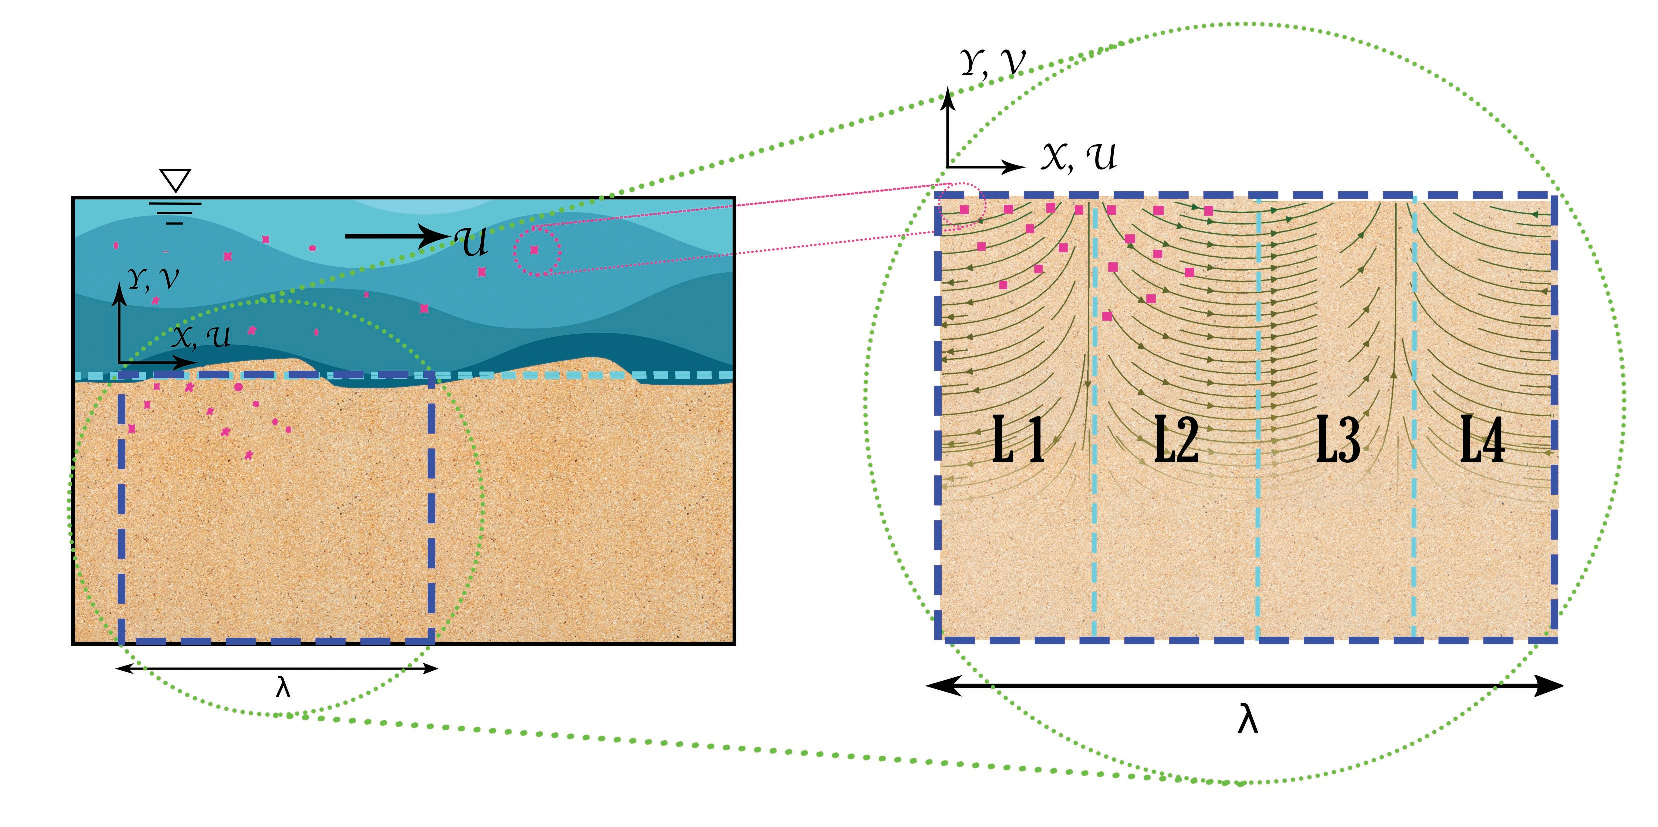
\includegraphics[trim=0.2cm 0.2cm 0.2cm 0.2cm, width=35pc]
{190404_ConceptualW.pdf}
\caption{Conceptual model for the posed problem. Left: Sand bed with dune shapes. The red box outlines the model domain ($\lambda$ is the characteristic dune's wavelength). The cyan dashed line demarcates the mean height of the bed. Right: Zoom of the model's domain. Idealized streamlines from velocity profiles. Note that the lateral boundary conditions of the model are periodic. Particles are seeded at the top of the domain in the first half of the dune wavelength.}
\label{Conceptual}
\end{figure}
% ============================================================================

% ============================================================================
% TABLE WITH PHYSICAL AND NUMERICAL PARAMETERS FOR THE PARTICLE-TRACKING
% MODEL THAT WAS PROPOSED
% ============================================================================
\begin{table}
\caption{Physical parameters \citep{Packman2000,Fox2014,Fox2018} for the comparison of the Particle-Tracking model implemented.}
\label{TF:Phys_Param}
\centering
\begin{tabular}{l c c}
\hline
PHYSICAL PARAMETERS						    & SYMBOL			& VALUE			\\
\hline
  Flume width $[cm]$  					    & $W$				& 29.0 			\\
  Sediment porosity $[-]$				    & $\theta$			& 0.33 			\\
  Hydraulic conductivity $[cm/s]$ 		    & $K$				& 0.12 			\\
  Flow $[l/min]$						    & $Q$				& 261.0			\\
  Mean stream velocity $[cm/s]$			    & $U$				& 15.0 			\\
  Crossection depth $[cm]$				    & $d_b$				& 20.0 			\\
  Dune wavelegth $[cm]$					    & $\lambda$			& 15.0 			\\
  Water depth $[cm]$					    & $d$				& 8.8 			\\
  Total streambed area $[cm^{2}]$		    & $A$				& 15.1	 		\\
  Imposed GW condition (in/out) $[cm/d]$    & $q_{in}$			& $\pm 12.5$	\\
  Filtering coefficient $[1/cm]$		    & $\lambda_f$		& 0.6			\\
\hline
\end{tabular}
\end{table}
% ============================================================================

The primary assumptions within the model are (i) macroscopic processes are considered separately from pore-scale processes, hence the movement of the particles is considered independent from the bed filtration process; (ii) particles do not interact with each other; (iii) particles do not change the flow conditions in the media when they are filtered in the bed; and (iv) fine particle deposition is irreversible. From experiments we know that these assumptions are not always valid, as particle colloisions can lead to larger agglomerates and particle clogging can alter flow paths \citep{Fox2018}. However, such processes add substantial complexity and can be added once the general model framework that we establish here is better understood. 

The horizontal model computational domain represents a single dune wavelength ($\lambda$) (figure \ref{Conceptual}). In the vertical axis, the domain has a side $d_b$ that stands for the depth of the sand bed, or the distance between the free surface flow and an impervious layer at the bottom of the domain. For practical purposes the width of the sand bed was modeled according to experimental values reported in literature \citep{Fox2014,Fox2018}. The sides of the box are open and they represent periodic boundary conditions as particles that exit the domain on the right will re-enter on the left boundary and viceversa (figure \ref{Conceptual}). 

The free surface model flow conditions are estimated by superimposing the advective pumping model \citep{Elliott1997} with each groundwater flow condition (i.e., losing, neutral or gaining). This model estimates the velocity field within the bed as a result of pressure variations at the top of the sand dunes that form the river bed. The particles are seeded at the top of the domain in the left half ($\lambda / 2$) of the domain, which conceptually represents the upstream (stoss) side of the sand dune. Each timestep, the introduced particles travel according to the estimated velocity field followed by a filtration process estimated using a random number generator. Subsections \ref{Mathematical_model} and \ref{Numerical_model} will explain in detail the particle mobility and trapping/filtering features of the model.

\subsection{Mathematical Model} \label{Mathematical_model}

The velocity fields used to model the water flow inside the dune are taken from existing literature \citep{Elliott1997,Packman2000} with an additional superimposed groundwater flow component  (equations \ref{u} and \ref{v}). The groundwater vertical flow condition is added to the existing profiles (i.e. positive upwards velocity for the gaining condition and negative downwards velocity for the losing condition) through the following equations: 

% Velocity profile equations - From Packman et al. 2000
% use \nonumber if you want to split an equation in different rows and not number a row
\begin{eqnarray}
\label{u}
  u & = & -(kKh_{m}) \cos(kx) [\tanh(kd_b)\sinh(ky) + \cosh(ky)] \\
\label{v}
  v & = & -(kKh_{m}) \sin(kx) [\tanh(kd_b)\cosh(ky) + \sinh(ky)] \pm q_{in/out} 
\end{eqnarray}

Where $x$ and $y$ represent the Cartesian coordinate reference axis ($y = 0$ is the top of the domain), $k$ stands for the normalized dune wavelength $(2 \pi / \lambda)$ and $u$ and $v$ for the horizontal and vertical velocity components, respectively. Furthermore, $h_m$ represents the mean pressure over the dune, $K$ stands for the permeability of the media, $d_b$ for the thickness of the bed that within the domain and $q_{in/out}$ is the component of vertical velocity caused by the groundwater inflow/outflow.

We normalized all of the quantities and parameters according to theory developed for flow and transport in sand beds \citep{Elliott1997,Packman2000}. As a result, equations \ref{u} and \ref{v} can be transformed in equations \ref{ustar} and \ref{vstar}. The inflow/outflow velocity $q_{in/out}$ is normalized by the maximum pumping velocity $u_m$. The addition of the vertical velocity alters the flow directions within the domain and introduces areas of flow recirculation and stagnation absent in the neutral flow condition velocity profiles (figure \ref{Velocities}a-c). The neutral velocity profile (figure \ref{Velocities}b) shows streamlines that are parallel among them, starting and ending in two vertical streamlines that enter and leave the domain at $-\pi/2$ and $\pi/2$. For the losing flow condition (figure \ref{Velocities}a) the vertical streamline that enters the domain at $\pi/2$ remains unaffected in its shape. However, the vertical streamline at $-\pi/2$ is cut due to the presence of the downward imposed flux. This feature generates a recirculation zone that enhances vertical downwards flux and hinders the upward flux that leaves the domain. Instead, for the gaining flow condition (figure \ref{Velocities}c), the vertical streamline located at $\pi/2$ and going downwards is cut and the streamline at $-\pi/2$ going upwards is enhanced by the groundwater flow condition.


% Dimensionless velocity profiles - From Packman with Elliott 
\begin{eqnarray}
\label{ustar}
  u^* & = & -\cos(x^*)[\tanh(d_b^*)\sinh(y^*) + \cosh(y^*)]\\
\label{vstar}
  v^* & = & -\sin(x^*)[\tanh(d_b^*)\cosh(y^*) + \sinh(y^*)] \pm q_{in/out}^*
\end{eqnarray}

% ============================================================================
% Velocity profiles - figure
\begin{figure}[ht]
\centering
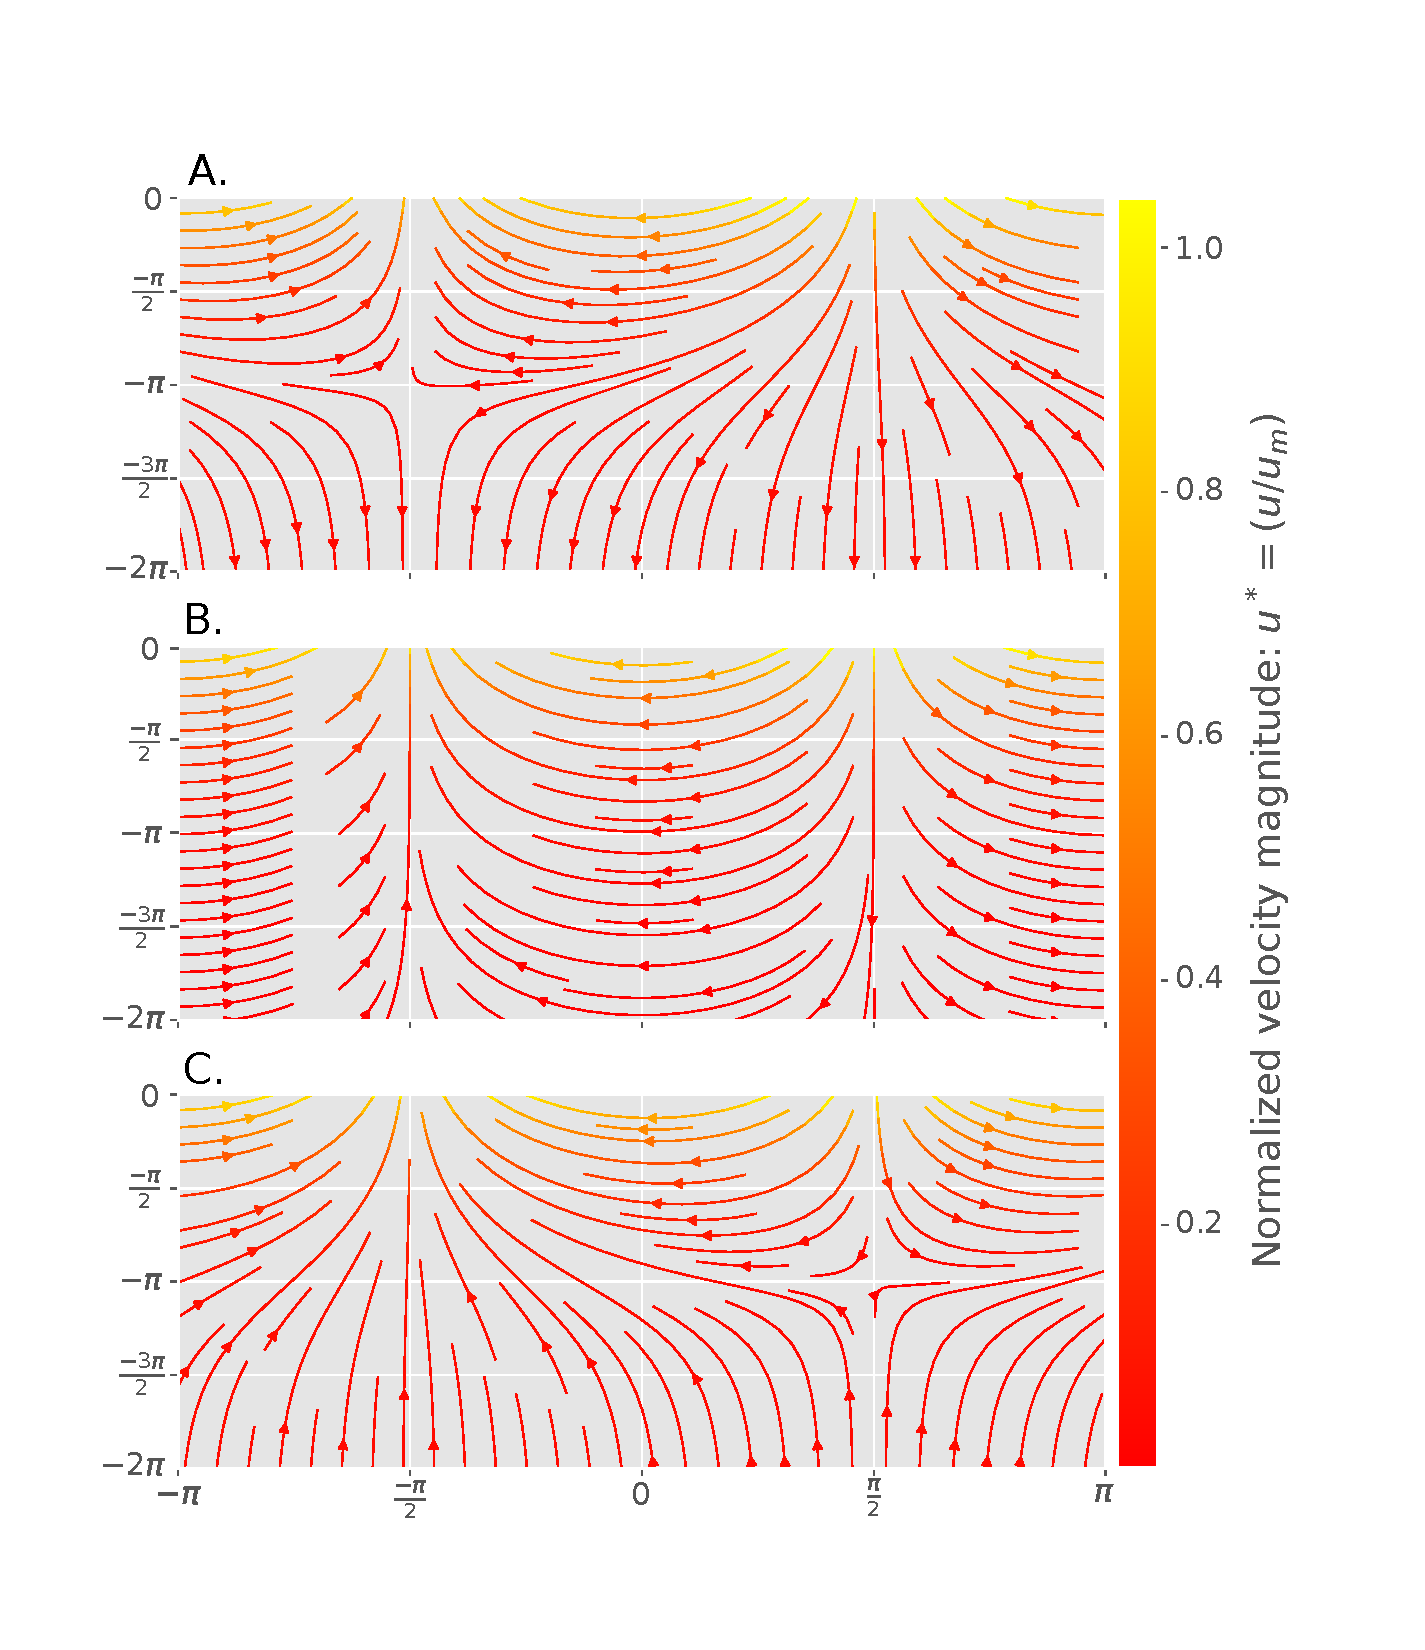
\includegraphics[width=35pc]
{190131_Streamlines.pdf}
\caption{Streamlines for (A) Losing, (B) Neutral and (C) Gaining flow conditions. Domains are plotted in the interval $[-\pi /2, \pi/2]$ since domain is periodic. The color bar represents the magnitude of the velocity vector. Vertical and horizontal axis not to scale.}
\label{Velocities}
\end{figure}
% ============================================================================

The resulting velocity profiles generated with the superposition of the advective pumping model and the vertical groundwater flow are physically reasonable, as the lowest velocities are present at the bottom of the domain where the low velocity groundwater flow is strongest and the highest are located close to the sediment water interface at the top of the domain. Moreover, the main dynamics of HE are not suppressed by the gaining/losing conditions imposed by the vertical groundwater flow.

Regarding the individual behavior of the particles, Stokes number is defined as the relation between the stopping distance and the characteristic length of the phenomenon \citep{Clark2009}. To understand the particle path behavior within the velocity profiles we compute the Stokes number (equation \ref{STK}) as:

% Stokes number calculation
\begin{equation}
\label{STK}
 	Stk = \frac{\rho_p d_p^2 u_0}{18 \mu_f l_0}
\end{equation}

Where $\rho_p$ is the particle density taken here as that of kaoline (2650 $\frac{kg}{m^3}$) \citep{NationalCenterforBiotechnologyInformation}, $d_p=384 \times 10^{-6} m$ is the mean diameter \citep{Fox2014},$u_0=0.01 \frac{m}{s}$ is the mean velocity in the subsurface (which is taken to be greater than the maximum obtained from equations \ref{u} and \ref{v}), $\mu_f=1.519 \times 10^{-3}Pa \ s$ is water's dynamic viscosity \citep{Cengel2006}, and $l_0=0.01 m$ is a characteristic length of the phenomenon which is similar to the dune height \citep{Fox2018}. The modeled clay particles follow the streamlines formed by the velocity profiles described in equations \ref{ustar} and \ref{vstar} as the computed Stokes number ($Stk=0.014$) is less than 1.0 \citep{Tropea2007}. The mathematical model starts with the transport of particles along given streamlines, i.e. the Advection Dispersion Equation (ADE) (equation \ref{ADE}). 

% Advection Dispersion Equation with just advection!!!!
\begin{equation}
 \label{ADE}
 	\frac{\partial C}{\partial t} \ + u \frac{\partial C}{\partial x} \ + \ v \frac{\partial C}{\partial y} \ = \ D \bigg(\frac{\partial^2 C}{\partial x^2} + \frac{\partial^2 C}{\partial y^2}\bigg) - S
\end{equation}

Here, $C$ stands for the concentration of the particles, $u$ and $v$ for the horizontal and vertical velocities, respectively; $D$ for the mechanical dispersion coefficient and $S$ for rate of particles removal due to filtration \citep{Packman1997}. The dispersion process can be neglected in particle transport in porous media \citep{Mau1992}, so the ADE can be transformed into an equation that represents a filtration process over a given velocity field (equation \ref{ADE2}). Here, the material derivative of concentration equals the rate of removal of particles over time.

\begin{equation}
 \label{ADE2}
 	\frac{D C}{D t} \ = \frac{\partial C}{\partial t} \ + \ u \frac{\partial C}{\partial x} \ + \ v \frac{\partial C}{\partial y} \ = \ - S
\end{equation}

The rate of particle removal $S$ can be expressed with the aid of the filtration coefficient $\lambda_f$, the seepage velocity $U = \partial s / \partial t$ (where $s$ is the path traveled by the particle), and the concentration $C$ of the analyzed particles as follows:

\begin{equation}
 \label{lambdaf}
 	S = \lambda_f \frac{\partial s}{\partial t}C
\end{equation}

When replacing the value of $S$ of equation \ref{lambdaf} in equation  \ref{ADE2}, the expression for particle filtering becomes: 

\begin{equation}
 \label{filtration}
 	\frac{\partial C}{\partial s} = -\lambda_f C
\end{equation}

This model formulation is consistent with previous models of colloidal transport in porous media \citep{Domenico1998}. The key outcome of the mathematical model is that a filtration process along steady streamlines can be expressed as a first order reaction. 

\subsection{Numerical Model} \label{Numerical_model}

The proposed numerical model is similar to the one used by \citet{Packman2000}. Its logical process is divided in three parts that use the discrete versions of equations \ref{ADE2} and \ref{filtration}. The initial step calculates the displacement of particles using the Taylor series expansion $\bar{x}(t + \Delta t) = x(t)  + u \cdot \Delta t$ \citep{Li2017}. Each timestep the model takes into account the particles' previous positions and determines their velocities based on the velocity field. 

After estimating each particle's position, the filtration process over the timestep is estimated calculating the probability $p$ that the particle stops inside the domain \citep{Prickett1981}:

% Simplification of the continuum - from eulerian to particles
\begin{equation}
\label{Filt_disc}
	p = 1 - e^{-\lambda_f \Delta s} \approx \lambda_{f} \Delta s
\end{equation}

This assumption holds since the size of the timestep $\Delta t$ is small enough to ensure the validity of the Taylor's expansion \citep{Li2017}.At the end of every timestep particles within the domain are counted and divided into two categories: (i) filtered particles that will remain immobile for the remainder of the simulation; and (ii) mobile particles which yet to be filtered. Particles that leave the domain out of the top boundary are accounted for as escaped particles that do not return to the domain during the simulation.

The particle-tracking simulations were performed under similar conditions to the ones proposed in table \ref{TF:Phys_Param}. The cases were modeled with $2x10^5$ particles for each vertical flow condition imposed (Losing, Neutral and Gaining). The total simulation time ensured that all of the seeded particles were either filtered or escaped the domain by the end of the simulation. As regards to the initial condition, the particles are seeded evenly distributed on the left half of the top of the domain ($0 < x^* < \pi$) within the imposed downwelling flow. Particles are not seeded on the right part of the domain ($\pi < x^* < 2\pi$) as the upwelling flow results in the particles immediately escaping the domain  \ref{Velocities}. 

% About the relative concentration windows where the results are analyzed.
To compare the PT model with the expeirmental results \citep{Fox2014,Fox2018}, the model domain is superimposed with a mesh of $100 x 167$ squares of size $\pi / 50$. Then, particles are binned and counted in each square. The resolution of the mesh was selected visually to ensure that results were representative for every one of the three modeled cases. It is worth mentioning that the mesh used for counting particles has no relationship with the computational PT simulation as it is only used for particle counting purposes \citep{Xue2017}.

% ============================================================================
% RESULTS SECTION
% ============================================================================
\section{Results}  \label{Results}

% 0. VELOCITY PROFILES UNDER DIFFERENT CONDITIONS WHEN SOLVING FOR THE DIFFERENT IN/OUT VALUES
The velocity profiles that result from equations \ref{ustar} and \ref{vstar} (figure \ref{Velocities}) show substantial differences among them. Preferential flow paths going upwards or downwards occur when the imposed condition is a gaining or losing flow, respectively. The addition of vertical flow (losing/gaining) to the neutral flow condition creates an area of no net flow. In addition, there is a corresponding recirculation zone in the losing and gaining cases (locations can be seen in Figure \ref{Velocities}A and C). These velocity profiles closely match those observed in the flume experiments with gaining and losing flow by \citet{Fox2018}.

Due to the altered losing and gaining flow, the maximum velocities in each profile are located in different places. In particular, in the losing condition the maximum velocity is into the bed (negative) on the stoss side (upstream) of the domain, while in the gaining case it is located in dune's lee (downstream). However, in the neutral condition the maximum velocities are located in two parts of the domain but with opposite directions, with downwelling on the stoss ($-\pi /2$) and the upwelling on the lee ($\pi/2$) side. Even though particles follow the streamlines of the velocity profiles, their deposition is not uniform due to the inflow position on the upstream side of the domain (dune's stoss side) and filtering along the streamlines.

% ============================================================================
% Logarithm of concentration - figure
\begin{sidewaysfigure}
\centering
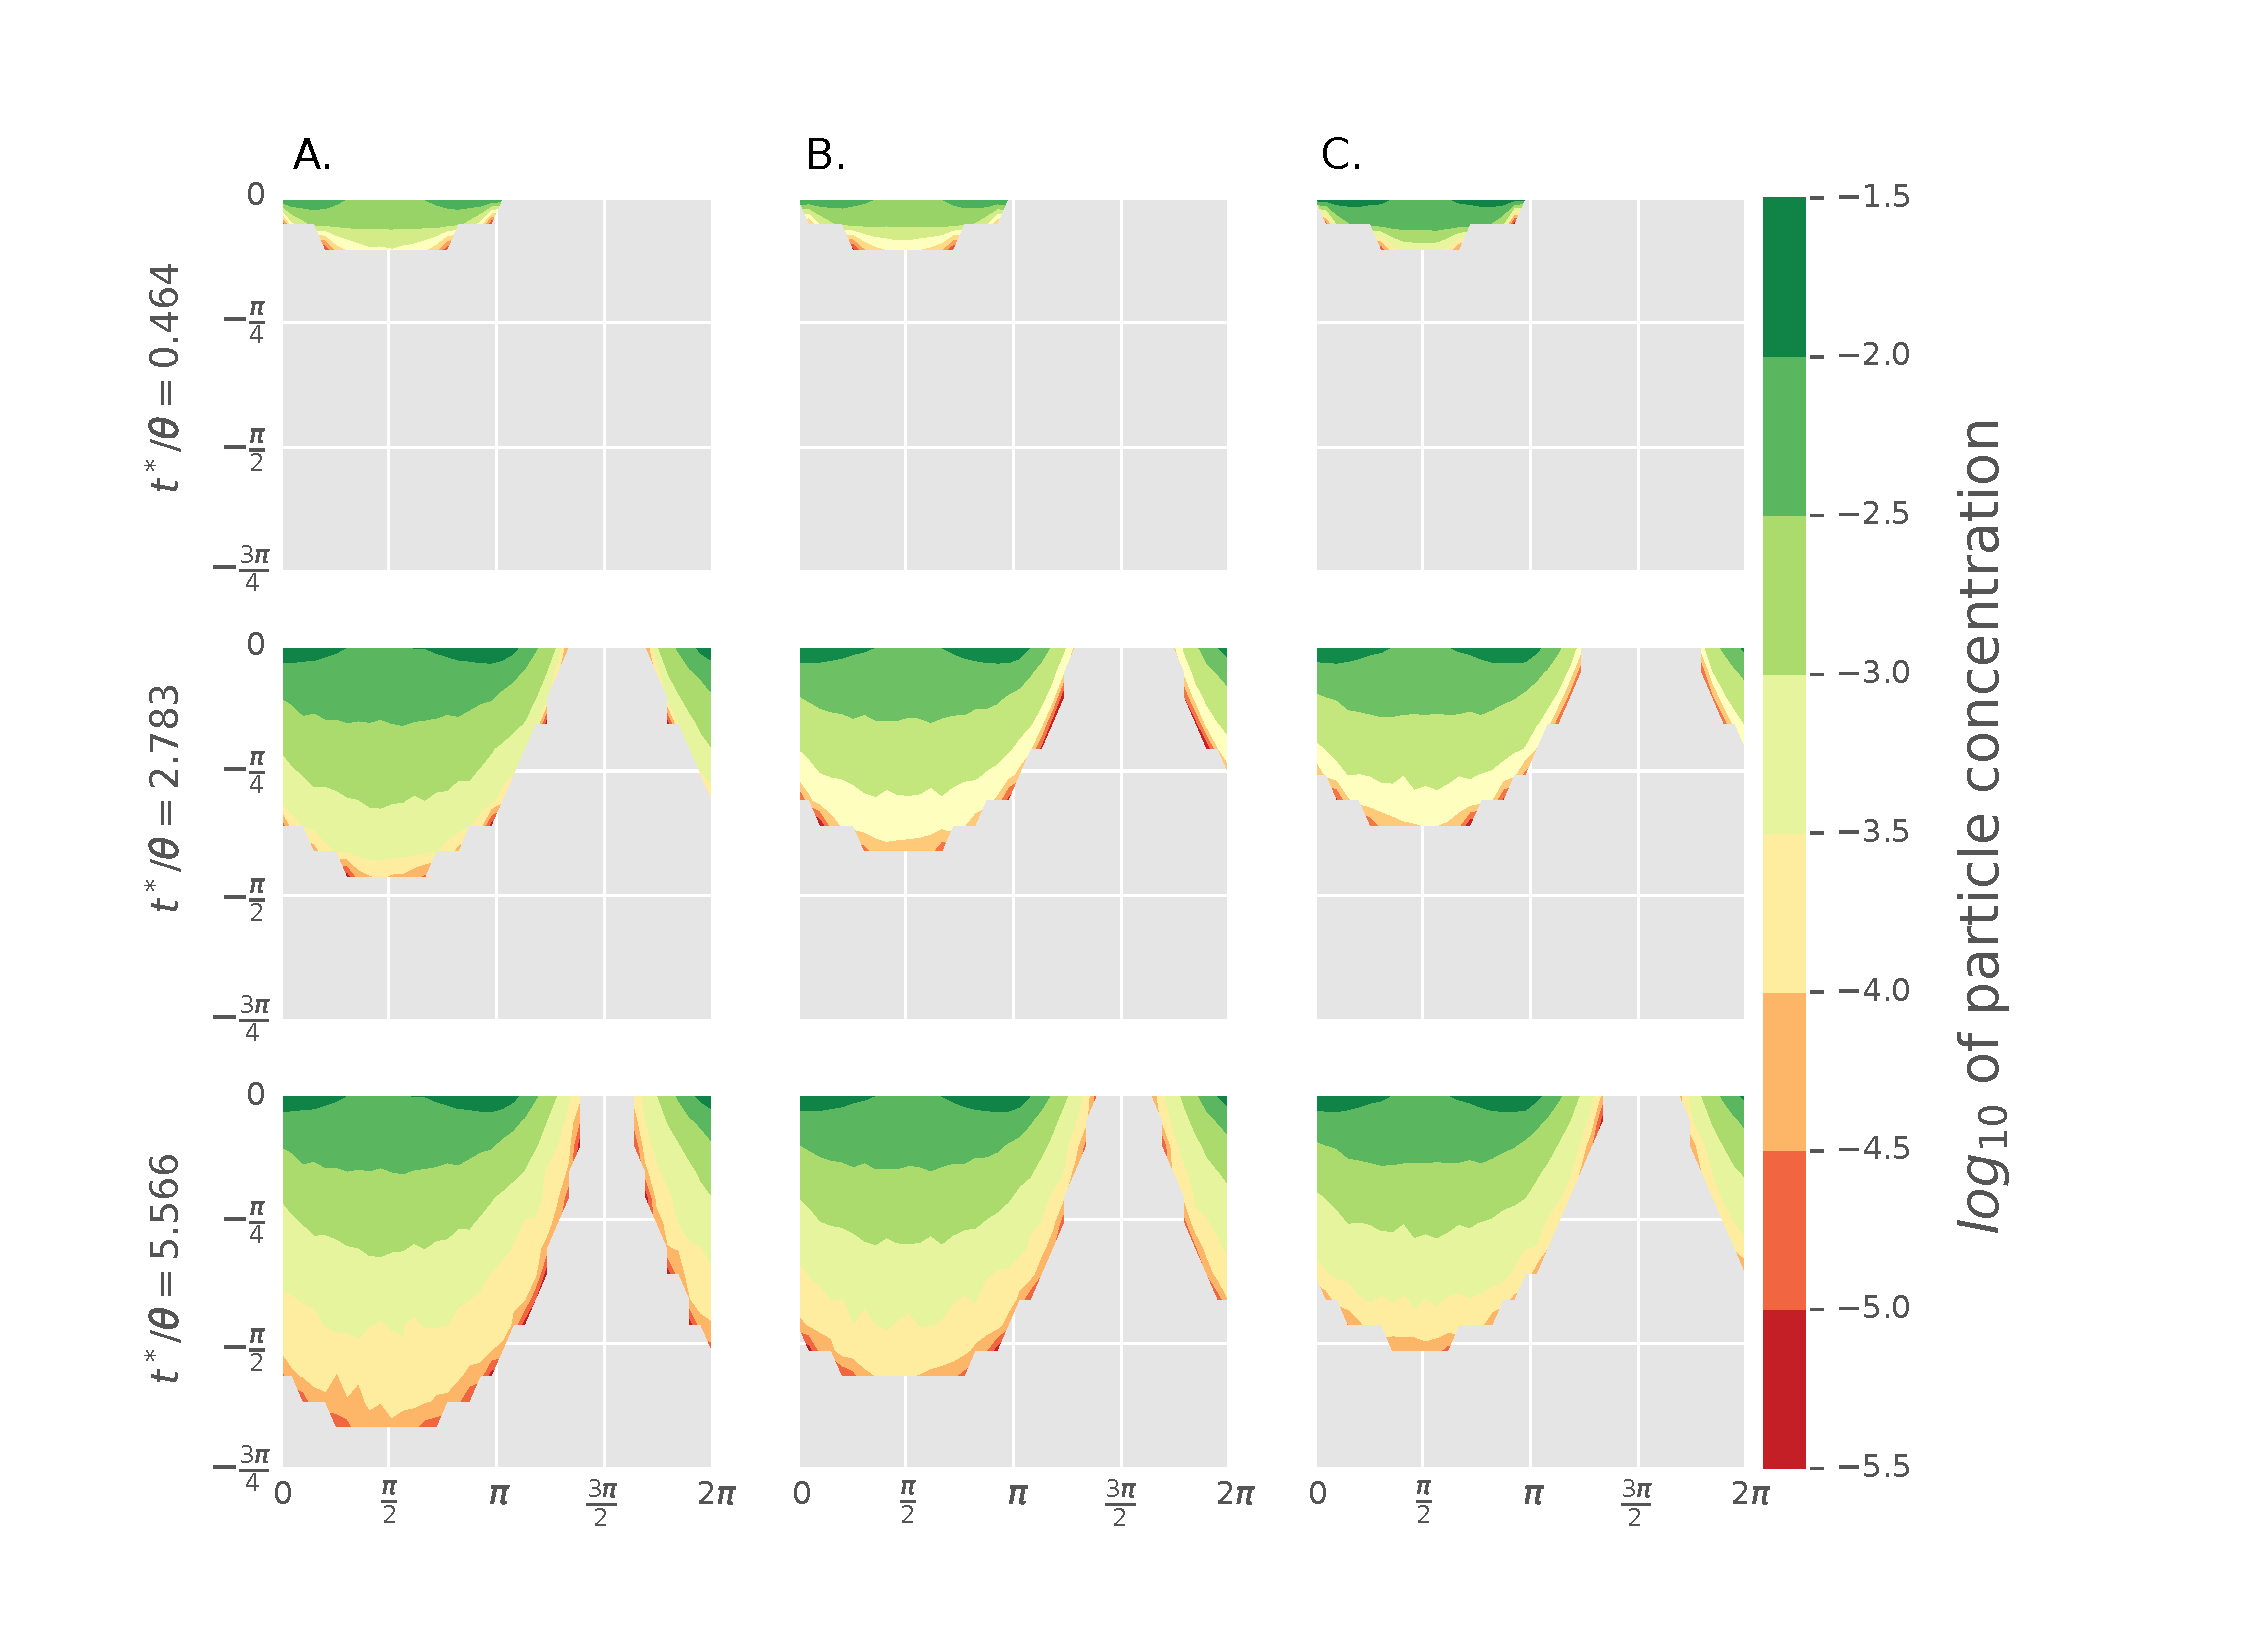
\includegraphics[trim=0.2cm 0.2cm 0.2cm 0.2cm, width=60pc]
{190131_Logplot.pdf}
\caption{Logarithm of total number of particles deposited for different times (rows), and under different inflow/outflow conditions (columns). (A) Losing condition, (B) Neutral condition and (C) Gaining condition (Note that axis are not to scale).}
\label{Logmap}
\end{sidewaysfigure}
% ============================================================================

Initially, the fine particle deposition pattern is generally similar, though the concentrations remain different between the analyzed cases (figure's \ref{Logmap} first row). For example, in the gaining condition the distribution of particles in the uppermost part of the domain is more evenly distributed than in the neutral and losing cases. At later times, the flow velocity pattern set up by the advective pumping flow remains prominent as the area of return flow is free of particles.  However, this gap is modified by the imposed vertical flow conditions; in the losing case the gap is significantly narrower than in the neutral and gaining ones (figure \ref{Logmap}). 

% 2. BEHAVIOR OF PARTICLES' IN TIME - HOW THEY GET DEPOSITED AND recirculated IN TIME ACCORDING TO THE FLOW CONDITIONS
With the PT model we can  assess the particles behavior over time (figure \ref{Pvst}), because we record the relative number of mobile, filtered, and escaped particles within the domain (figure \ref{Pvst}). In particular, even though each flow condition has the same filtering coefficient, the amount of particles that remain in the domain and escaped from it varies significantly between the imposed vertical flow conditions. The particle behavior over time for each modeled case is unique, i.e. each one of the vertical flow conditions has characteristic curves of filtered, mobile, and escaped particles (figure \ref{Pvst}). For the losing case the maximum fraction of filtered particles by the end of the simulation is $0.82$; while it is $0.78$ and $0.76$ for the neutral and gaining cases, respectively. Regarding the fraction of particles that escaped the domain, values of $0.17$, $0.20$ and $0.24$ are reported for the losing, neutral and gaining cases, respectively.

% ============================================================================
% Particles in time - figure
\begin{sidewaysfigure}
\centering
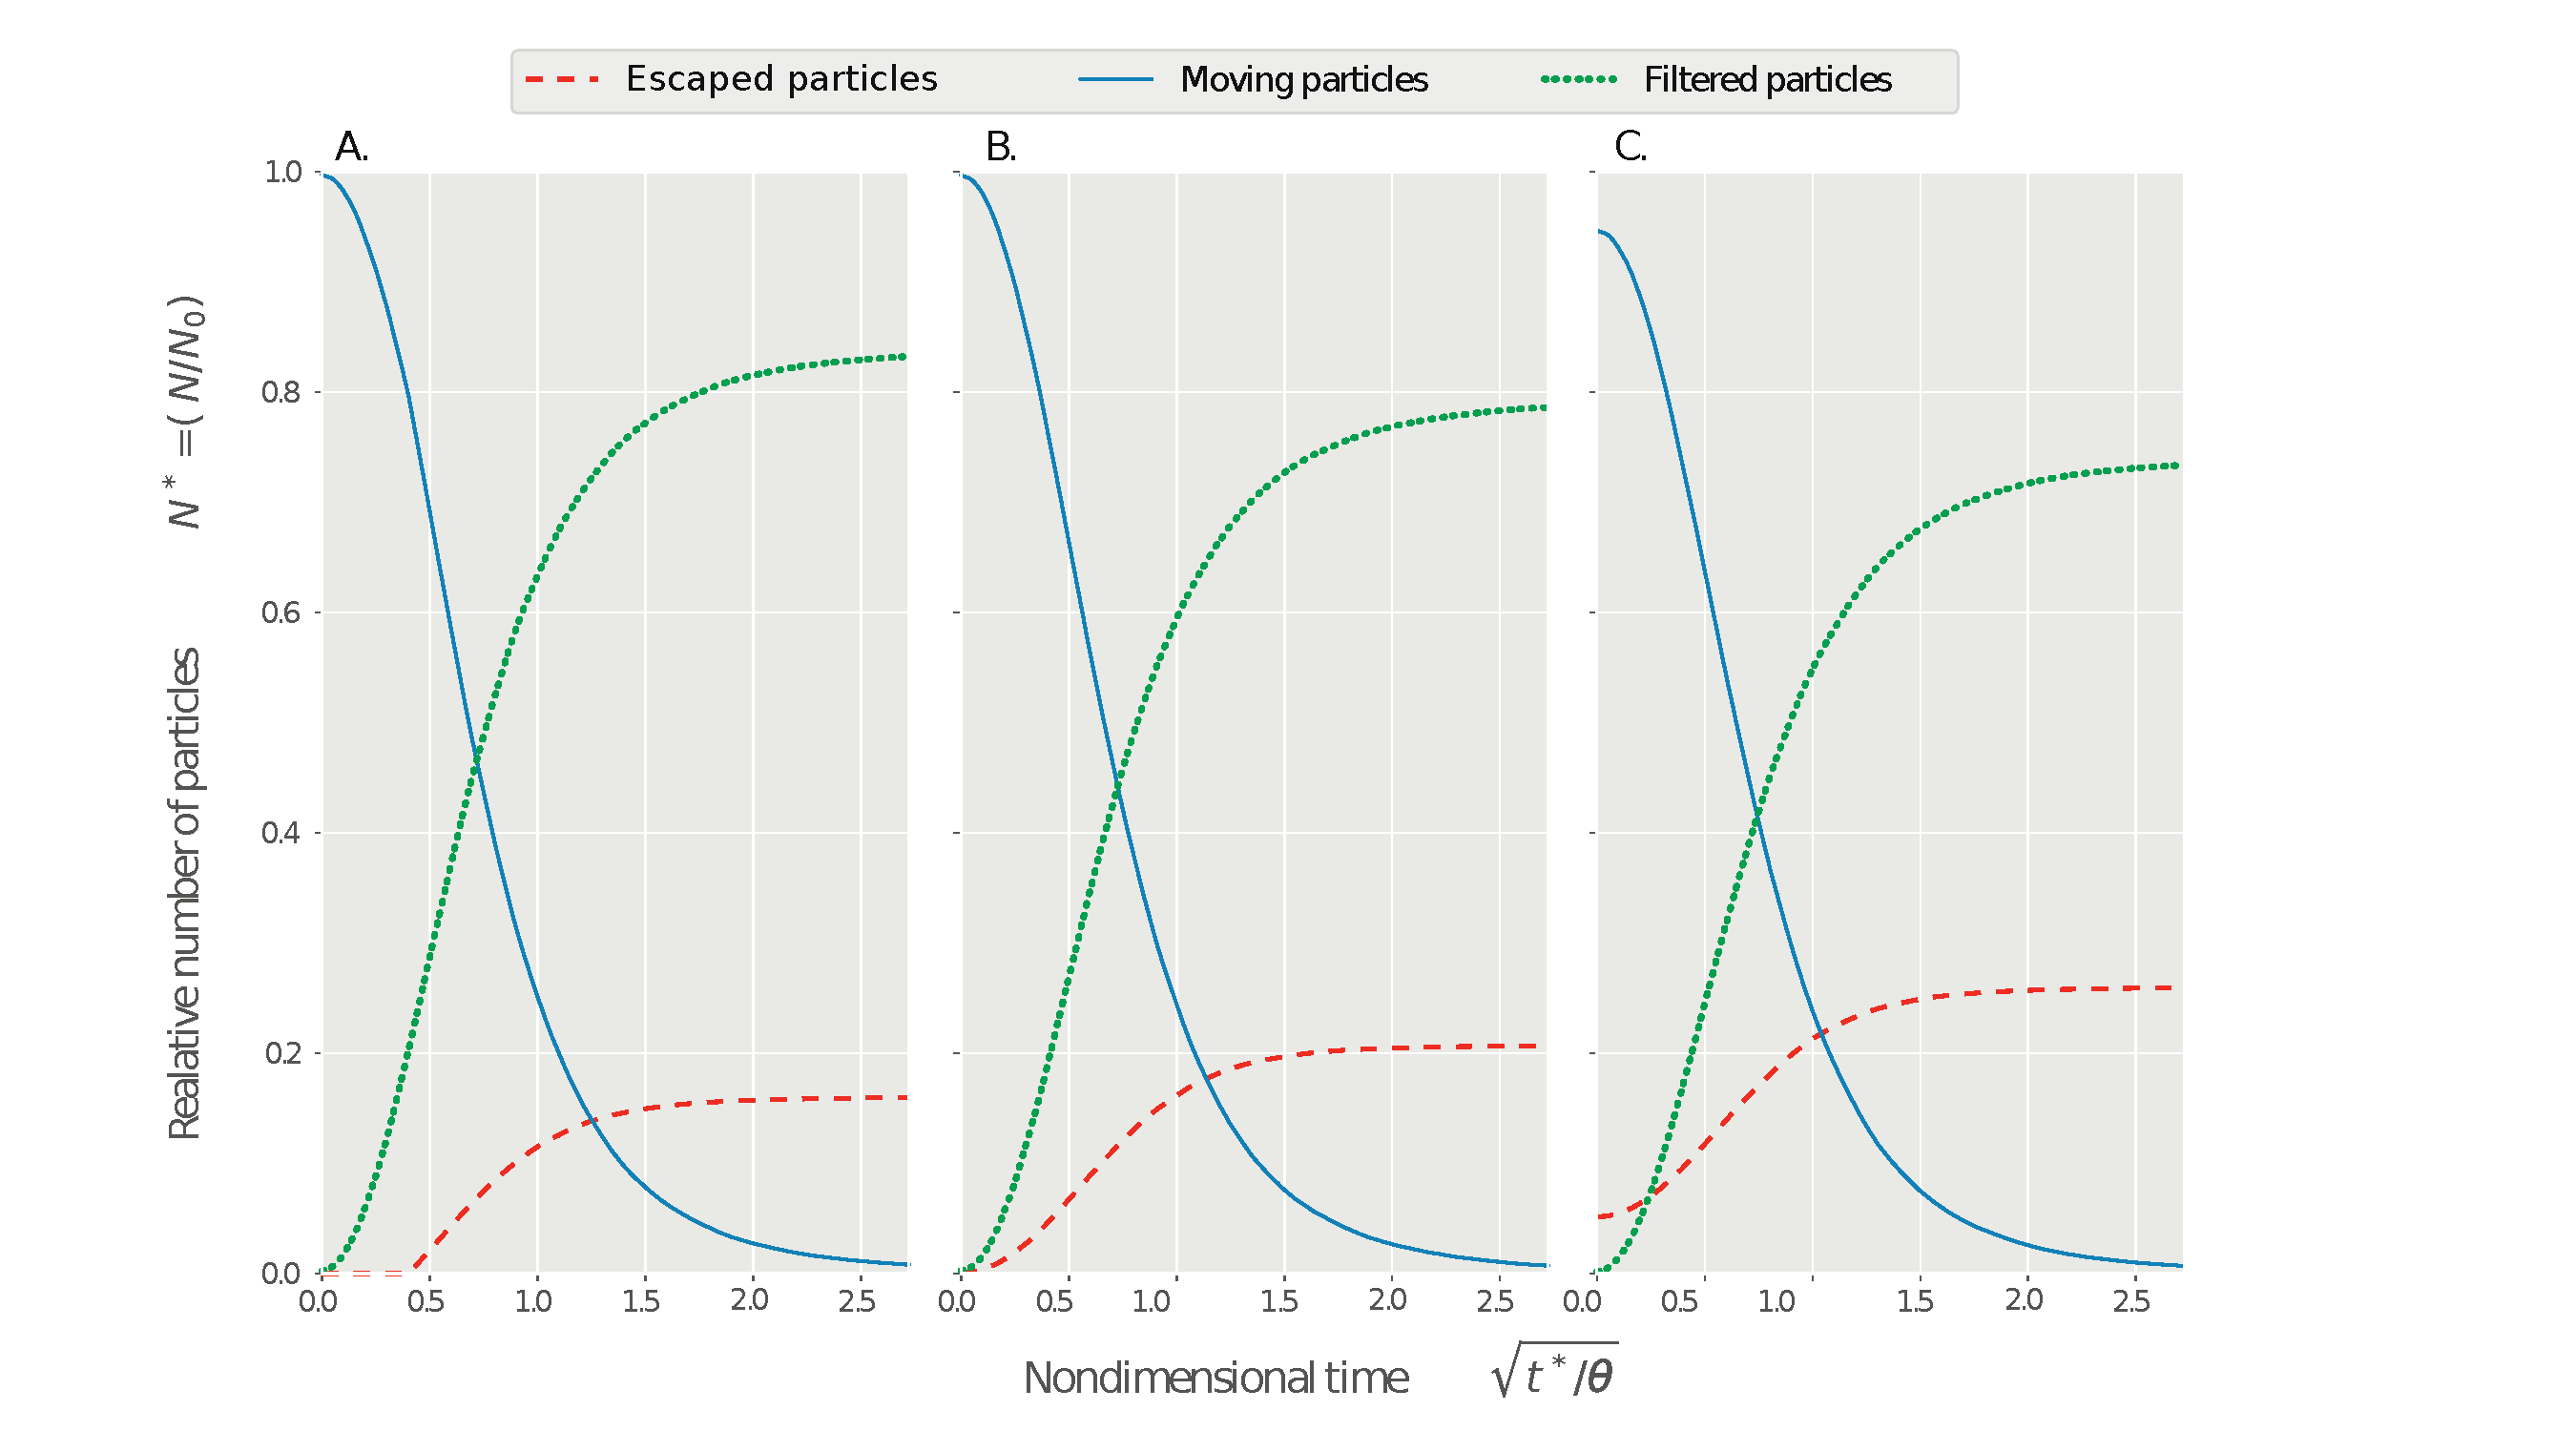
\includegraphics[trim=0.2cm 0.2cm 0.2cm 0.2cm, width=60pc]
{190305_Pvst.pdf}
\caption{Behavior of escaped (Red line), moving (blue line), and filtered (purple line) particles over time. (A) Losing condition. (B) Neutral condition and (C) Gaining condition.}
\label{Pvst}
\end{sidewaysfigure}
% ============================================================================

The PT model recovers the expected ensemble continuum behavior of fine particle deposition. The filtration process is expected to remove particles in an exponential way and the model is representing this phenomenon. Indeed, this decrease corresponds to the exponential decrease that results from solving equation \ref{Filt_disc} \citep{Li2017}. However, the presence of particles inside the domain is heavily conditioned by the vertical groundwater flow imposed. Indeed it is determined by the joint effect of both filtration coefficient and imposed vertical groundwater flow.  

% 4. RESIDENCE TIME AND PORTION OF PARTICLES INSIDE THE DOMAIN AT ANY GIVEN TIME.
By tracking the number of remaining particles within the PT model we can estimate a Residence Time Function (RTF). We calculate the RTF as the fraction of particles that enters the bed near $t = 0$ and remains inside the domain after a given time $\tau$ \citep{Elliott1997,Packman2000}. For small times, $\tau$ close to zero, the value of the RTF is $1.0$, as $\tau$ increases some of the particles leave the domain and the RTF begins to decrease. Since the RTF is normalized by the total number of particles (figure \ref{RTF}), the resulting curve is interpreted as the cumulative distribution function (CDF) of particles inside the domain. Moreover, as the filtration process within the PT model is irreversible, the RTF can never be equal to zero.

% ============================================================================
% Residence time function - figure
\begin{figure}[ht]
\centering
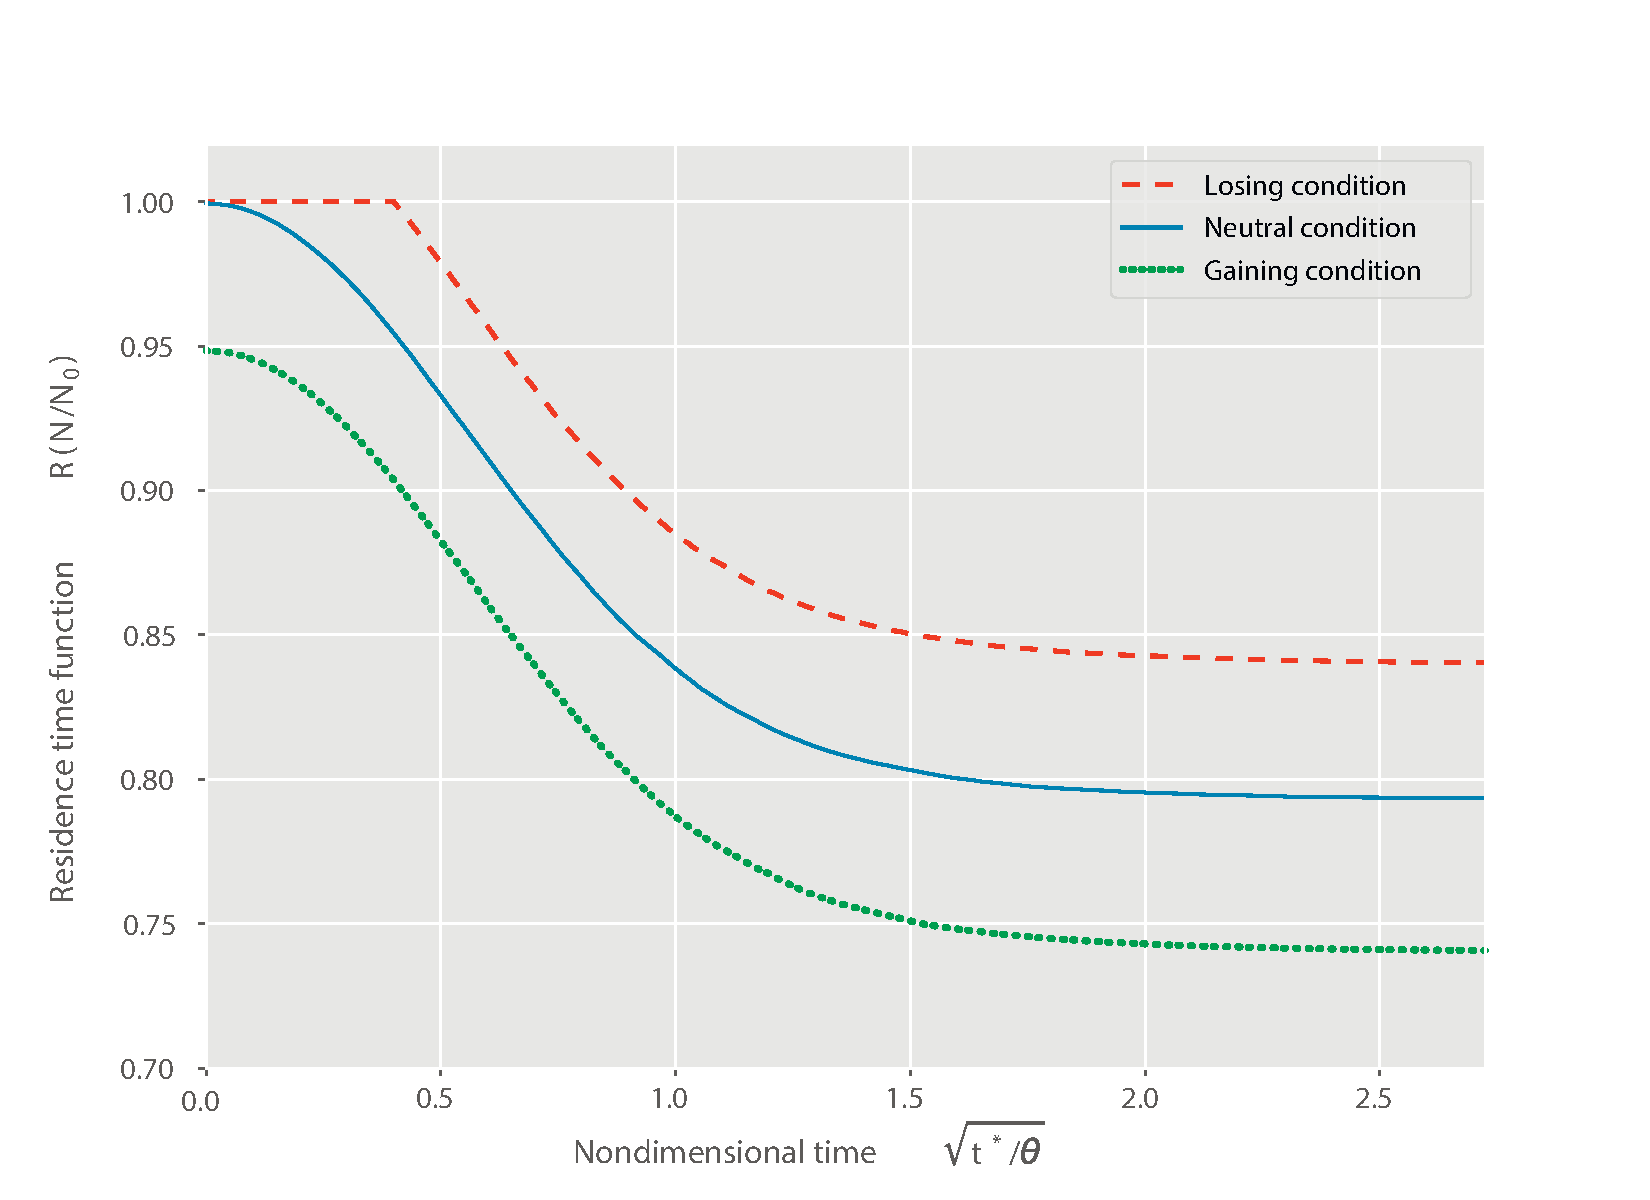
\includegraphics[trim=0.2cm 0.2cm 0.2cm 0.2cm, width=35pc]
{190305_RTF.pdf}
\caption{Residence time function for the different imposed flow conditions. The lines represent the Cumulative Distribution Function (CDF) of particles inside the domain at a time $\tau$ after the injection.}
\label{RTF}
\end{figure}
% ============================================================================

% 5. Residence time function and the derivative (check when the other model is run)
The number of particles remaining within the domain depends on the vertical flow conditions. Under the losing flow conditions particles encounter longer flow paths resulting in more time within the domain and an increased likelihood of filtration by the sand bed. For all time scales, neutral and gaining flow conditions have RTFs with very similar forms, although under gaining flow fewer particles enter the bed from the start. Unlike the neutral and gaining flow conditions, under losing flow the RTF remains constant for a short period where all particles enter the bed and none have recirculated yet. At longer timescales each RTF approaches a constant value. Although gaining and losing conditions have the same value but a different flow direction, the results of the RTF for the losing and gaining conditions are not equally distant from the RTF curve of the neutral condition. The losing condition RTF is closer to the neutral condition than the gaining one. To explore this, the rate of change of the RTF in time was estimated for the three cases (figure \ref{RTFder}). These curves are the Residence Time Distribution (RTD) and were obtained by taking the gradient of each RTF and then applying a convolution between the derivative and a top hat function with unit area and a span of $400$ points. 

% ============================================================================
% RTF der - figure
\begin{figure}[ht]
\centering
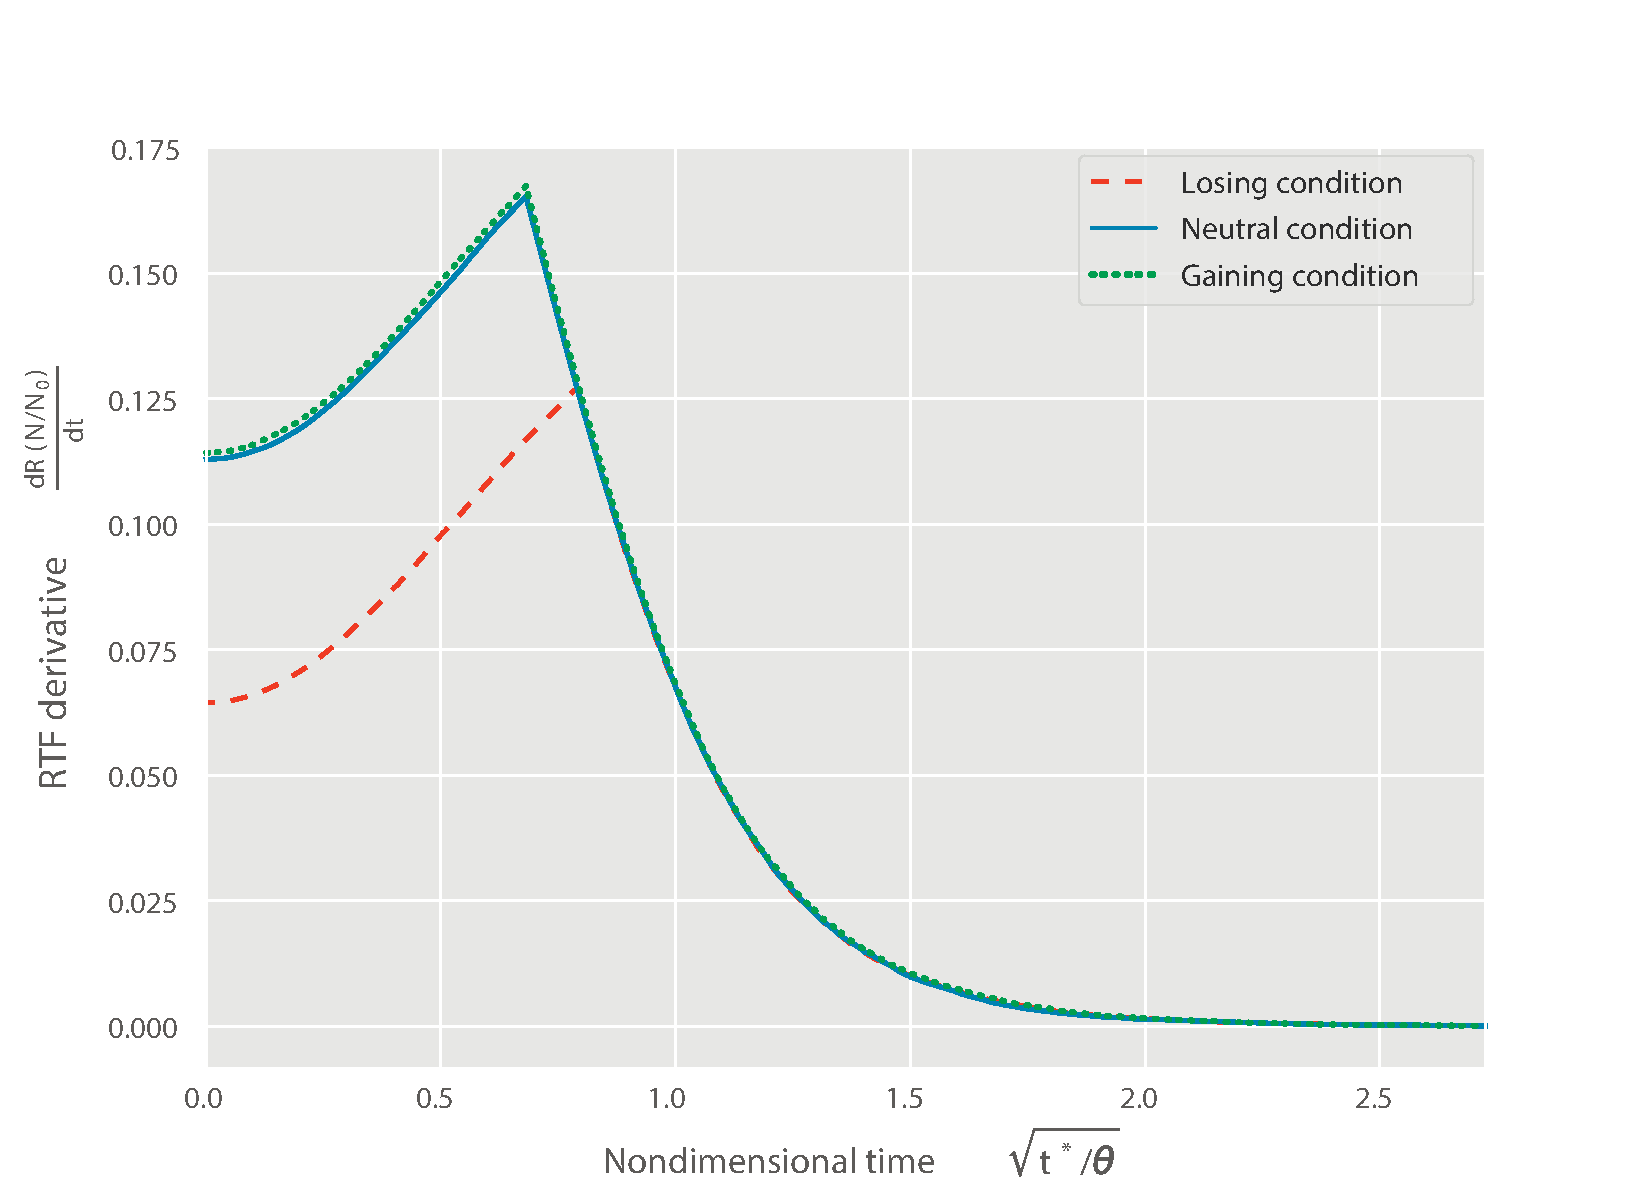
\includegraphics[trim=0.2cm 0.2cm 0.2cm 0.2cm, width=35pc]
{190305_RTF_der.pdf}
\caption{Derivative of RTF for the three vertical groundwater flow conditions modeled. These lines represent the Probability Density Function (PDF) of particles inside the domain at a given time $\tau$ after injection}
\label{RTFder}
\end{figure}
% ============================================================================

The time it takes the RTF to decrease at early times corresponds to the minimal path that a particle can travel through the domain before exiting at the surface. For the losing case, this path is longer than for the neutral and gaining cases. This aspect of longer flow paths is also reflected in the RTD for the losing case (figure \ref{RTFder} red line), which starts with a lower probability of particles leaving the domain and a maximum probability that is remains lower than the other two flow conditions. For all modeled cases, the probability of a particle leaving the domain is low at early times followed by an increase until the peak and then a monotonic decrease until all particles are removed or filtered. The primary difference between the three conditions occurs before the peak in the RTD probability, after this point the three distributions are nearly identical (figure \ref{RTFder}).

% 6. COMPARISON BETWEEN NUMERICAL AND EXPERIMENTAL RESULTS FORM FOX'S PAPER
We compare the PT model output with the experimental results from \citet{Fox2014,Fox2018}. Experimental subsurface particle deposition was sampled by coring each dune in triplicate at four equally spaced locations (\ref{Conceptual}c). Clay mass was estimated from the extracted cores at $0.5 \ cm$ intervals for each location, however at some depths clay concentrations were below detection limits or absent. To facilitate the comparison between the experimental results and the PT model, we divide the non-dimensional domain into sections of $\pi/2$ width. We then calculate the mean and standard deviation of the relative number of particles at each location. Accordingly, the mean mass fraction of clay is compared with the mean relative number of particles in every location and the standard deviation of the experimental measurements is compared with the standard deviation of the relative number of particles (figure \ref{Comparison}). The comparison of the experimental and the PT model results indicates that there is similar behavior in the decrease of fine particle concentration with depth for the three flow conditions, particularly in locations 1 and 2 (figure \ref{Comparison}).  

% ============================================================================
% Comparing with experimental results - figure
\begin{sidewaysfigure}
\centering
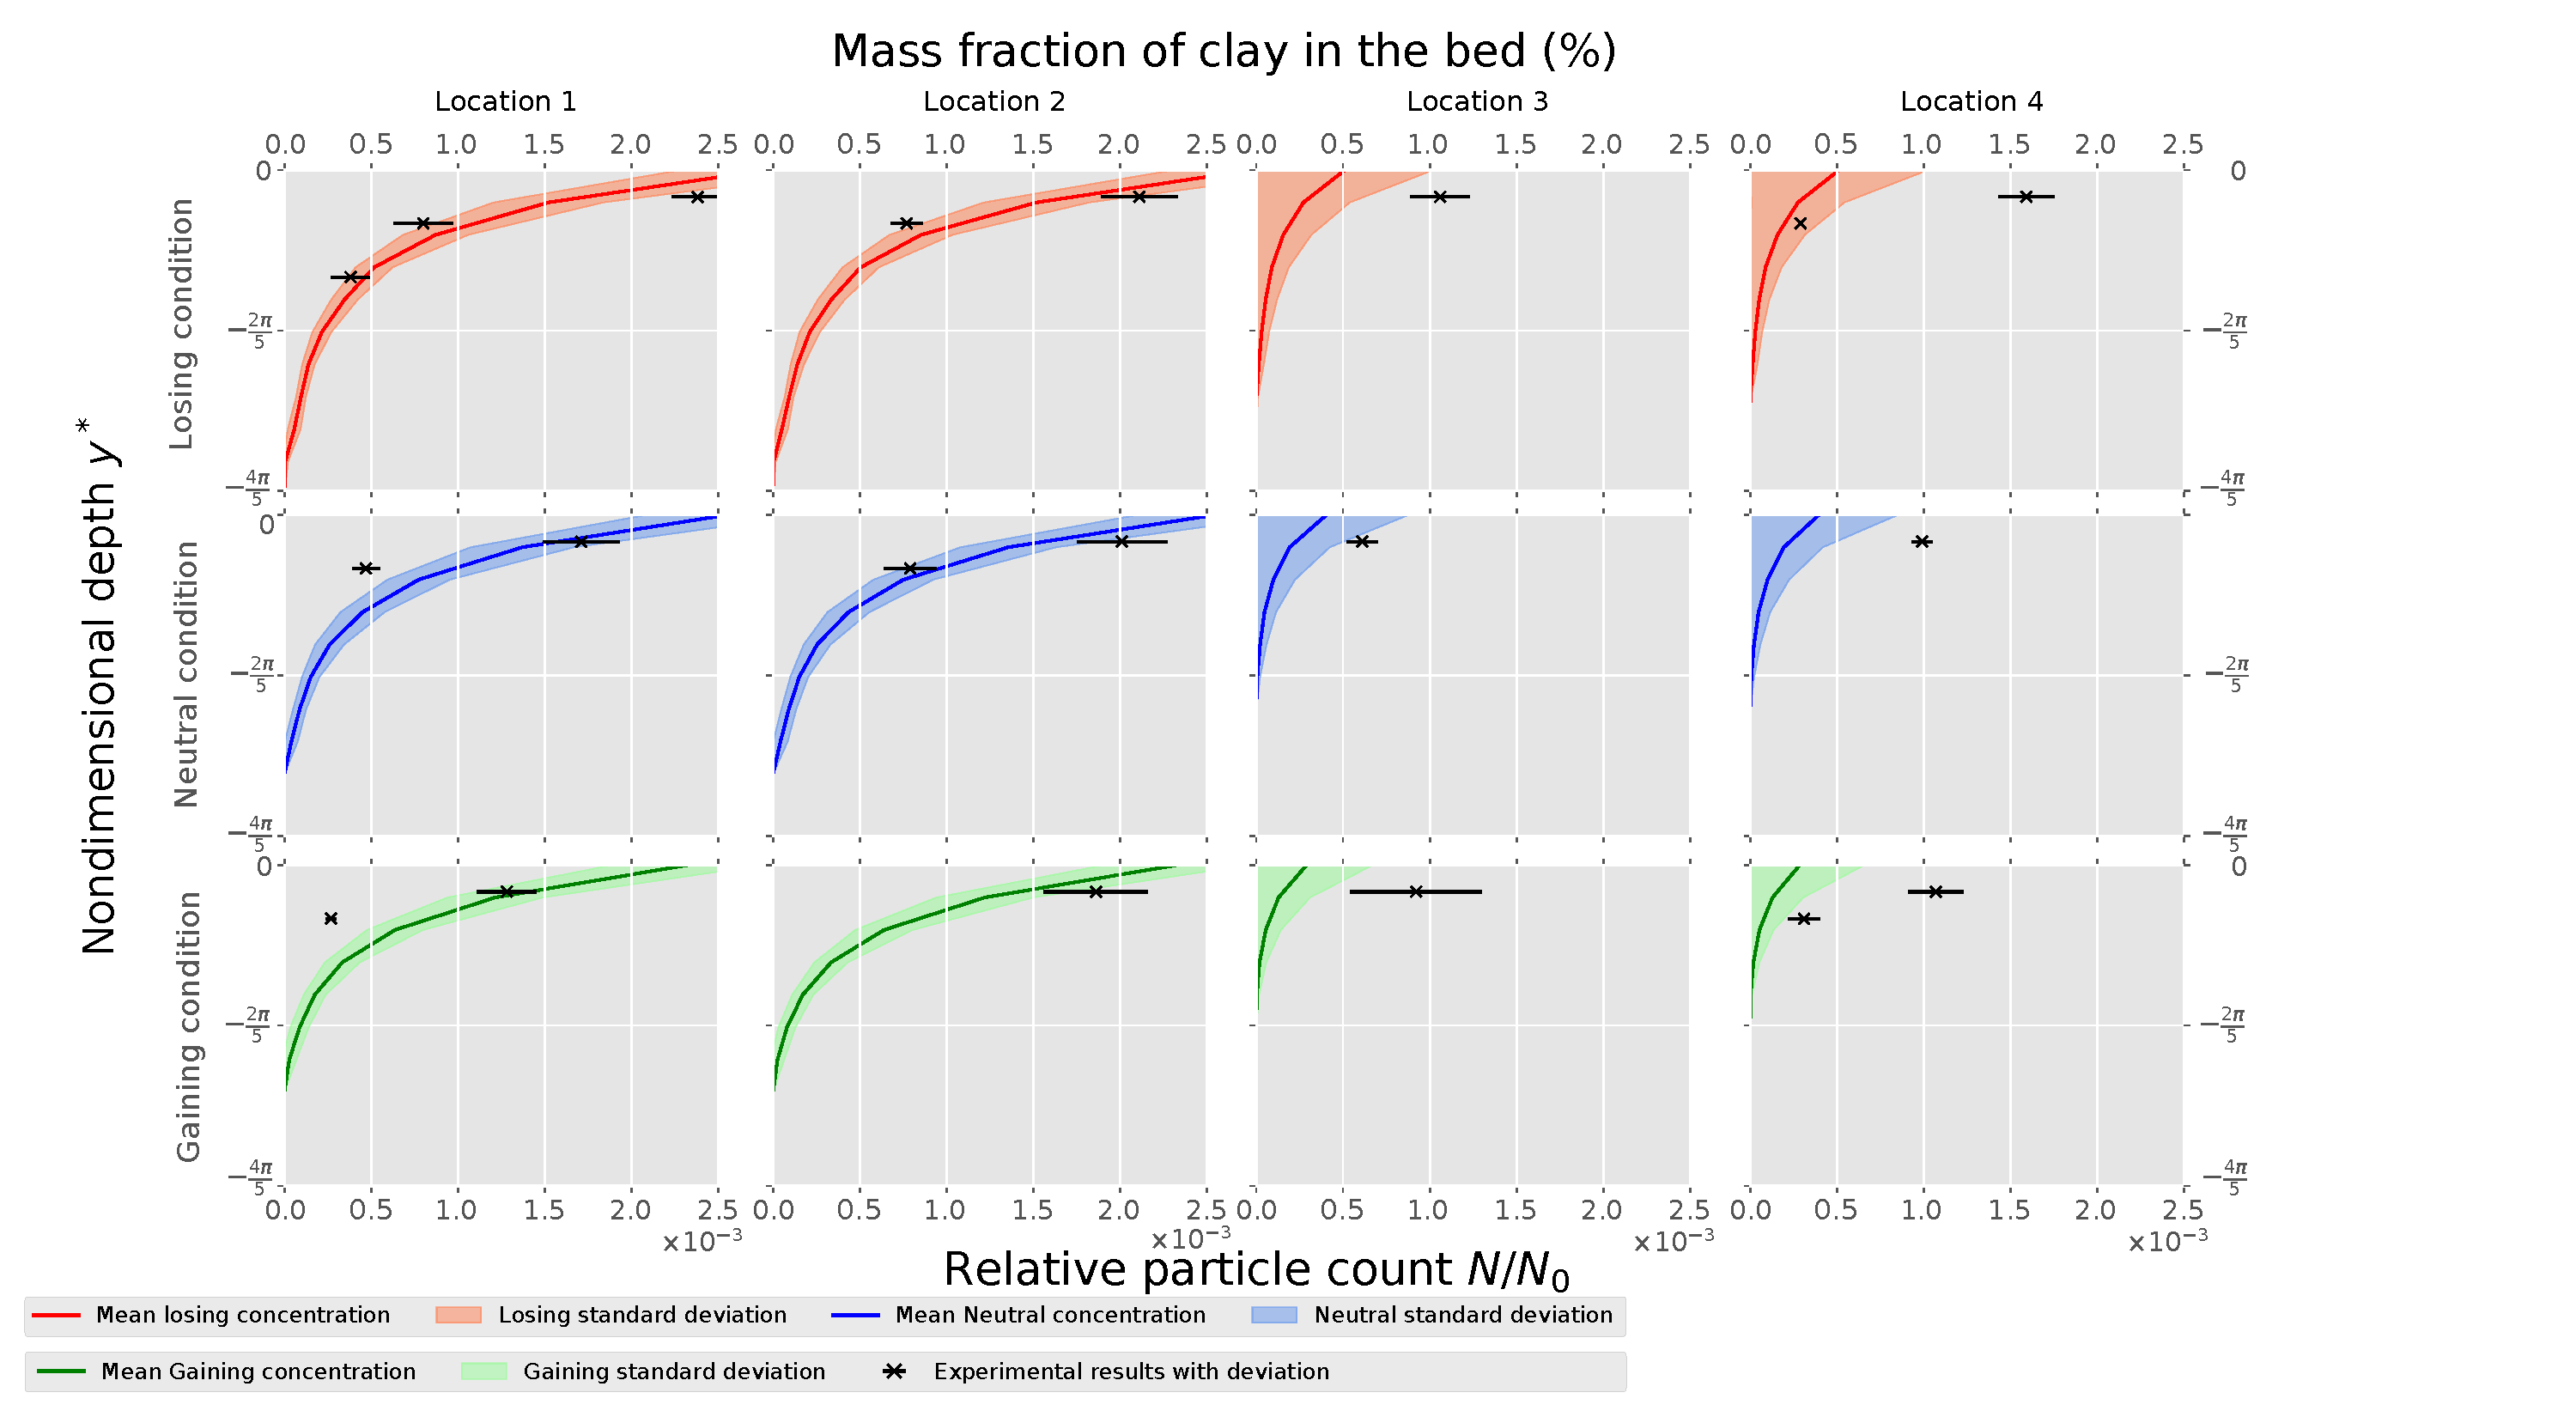
\includegraphics[trim=0.2cm 0.2cm 0.2cm 0.2cm, width=65pc]
{190131_Comparing.pdf}
\caption{Comparison with experimental results from \citep{Fox2018}. The top horizontal axis represents the fraction of clay mass found in the experiments expressed in $\%$. The bottom horizontal axis represents the fraction of particles within the numerical domain. Solid colored lines and their corresponding shaded areas represent the average fraction and standard deviation of particles at each depth for the different locations. Crosses are the mean mass fraction sampled in the experiments, and black lines represent the standard deviation of the measurements.}
\label{Comparison}
\end{sidewaysfigure}
% ============================================================================

Our results show strong similarities between the experimental results and the PT model, showing that fine particle deposition varies according to the location within the dune. Particles deposit more in locations one and two (the stoss side of the dune), and show reduced deposition in locations three and four (lee side of the dune). The deposition in the latter locations occurs due to the particles following the upstream (right to left) hyporheic flow paths (figure \ref{Velocities}). There is good agreement between the PT model and the experimental results in locations 1 and 2 of the sand dune (figure \ref{Comparison} first two columns). For each of the three flow cases modeled, the PT model underestimates the concentration of particles as the experimental results show more clay deposited with depth for locations three and four (\ref{Comparison}). Overall though, the similarities between the PT model and the experimental results highlight the impacts of filtration and vertical flow on particle deposition patterns. 

% ================================================================================
% DISCUSSION SECTION
% ================================================================================
\section{Discussion} \label{Discussion}

% 1. Velocity profiles and deposition patterns analyzed
The PT model developed here departs from an ADE and combines it with a stochastic filtration framework \citep{Li2017} to simulate fine particle deposition within a sand bed. This PT model framework does not pose any problems regarding mass conservation, artificial diffusion or unwanted oscillations provoked by numerical scheme instabilities \citep{Delay2005}. Additionally, the particle deposition and flow patterns are physically consistent with experiments and follow the expected mean continuum behavior, i.e. the model captures the physical processes in a representative scale by simulating the combination between the pore scale filtration and the macro scale due to the advective pumping flow. Therefore, the fine sediment deposition process can be divided into these basic two components.

The Stokes number for each individual particle is low enough that it is safe to assume that the particles follow the streamlines. This assumption is supported due to the size of a typical clay particle and the maximum velocity which it is subject to when entering the streambed. Because, the low Stokes number assumption is validated for the maximum velocity, it holds for all lower velocities (equation \ref{STK}).Consequently, the phenomenon of settling velocity inside the sand bed is not taken into account as it was in previous works \citep{Packman2000}.

The gaining flow condition produces less deposition than the neutral and losing condition (figure \ref{Logmap}). At early times the deposition is similar for all of the three modeled cases because the shallow streamlines have higher velocity, hence they are barely altered by the groundwater flow. But when particles travel to deeper parts, the groundwater and vertical flows become more important. The groundwater vertical flow imposed is estimated to be $8 \%$ of the maximum pumping velocity $u_m$ at the top of the domain. However, filtration is a function of each particle's displacement $s$, hence deposition is present only at the top of the domain in all of the modeled cases, because of the combination of velocity profiles generated by the dune shapes and the imposed vertical groundwater flow.

Important differences arise when comparing deposition patterns from the three conditions modeled as the depositional pattern depends on the subsurface velocity profiles. The deposition patterns (figure \ref{Logmap}), show that a change in the vertical flow conditions affect not only the maximum penetration depth of the particles, but also the horizontal extent of the particles. Not only will a greater degree of particles deposit under the losing flow condition, but the deposited particles will also cover a larger subsurface area than the  neutral and gaining cases (figure \ref{Logmap}). This explains the decay in hyporheic exchange in the experiments run with conservative tracers after clay injections under different vertical flow conditions \citep{Fox2014,Fox2018}. Namely, when fine particles cover a larger portion of the dune wavelength, the penetration of a conservative tracer is hindered because of the fine particle deposition. 

In addition, the PT model shows that the velocity profiles and filtration produce different particle concentration profiles. In other words, fine particle penetration is different for all of the modeled cases, depending on the imposed vertical groundwater flow. Therefore, fine particle penetreation in the bed is different for the different cases at different locations (continuous lines in figure \ref{Comparison}). These results show agreement with experimental results that clearly show an uneven distribution of clay mass in the dunes \citep{Fox2018}. The decay of mean clay concentration with depth is similar to the experimental results presented by \citet{Fox2018}, especially for the stoss side of the dune. Suggesting that to a first order, the mechanisms responsible for particle deposition within the PT model are responsible for fine particle deposition patterns. Agreement between the PT model and the experimental results is poorer for the lee side of the bedform and, in general, the PT model standard deviation is less than that of the experimental results. The increased variability within the experimental results may be explained by differences in shape of the dunes in the experiment and the proposed idealized dune within the numerical model.As our model simulates and idealized dune with a fixed shape and constant physical properties inside the domain. Additionally, within the laboratory experimental set up, the shape of the dunes and the bed porosity are not homogeneous due to heterogeneity within the initial conditions.  

% 2. WEAKNESSES AND HOW TO OVERCOME THEM
The numerical PT model flow conditions simulate an idealized flow, hence the effects of turbulent flows on the internal velocity profiles of the dunes are not taken into account in these types of models that use steady velocity fields for estimating the particles' position in every timestep. In natural and laboratory cases, some of the total fine particle deposition occurs due to turbulence because of its ability to transport mass and momentum from the free flow stream to the porous media \citep{Roche2018}. However, our model is able to capture the main fine particle deposition phenomenon, pointing out that even if turbulence plays an important role, the velocity fields and the filtration are main drivers for the depositional patterns.

In addition, changes in porosity (hence permeability) of the media due to the particles' deposition has been recorded in field observations (CITATION), affecting the shape of the velocity fields under the different flow conditions. The change of bed porosity hinders HE in rivers and has visible effects on different experiments \citep{Fox2018}. Furthermore, fine particle movement and deposition in the bed is also conditioned to the variable flow generated by the clogging of the bed. Nevertheless, our results suggest that this PT model is suitable to represent deposition patterns under different flow conditions, mainly at early times when the clogging processes have not yet affected the flow field significantly. For cases of dunes with more heterogeneous materials, the model could be adapted in order to capture the desired features. 

Finally, natural streams are characterized by their heterogeneity in space and time, hence our homogeneous sand bed PT model is not able to capture the fine particle deposition if compared to a more complex media made of different stratified materials like the ones found in natural streams. However, our results suggest that PT models remain a good approximation to the fine particle deposition phenomenon and that these type of models are a good approximation to understand how combined physical phenomena act as a whole in natural systems. 

\section{Conclusions} \label{Conclusions}

The implemented PT model is a useful tool to understand how two physical processes (i.e. bedform generated flow and filtration), control fine particle deposition in sand beds. The flow fields generated by both, flow over a dune and vertical groundwater flow, drive the fine particles inside the sand beds and generate irregular deposition patterns despite the constant ability of the bed to filtrate particles while traveling within the analyzed domain. Moreover, our results suggest that the observed irregular deposition patterns can result from the flow pattern alone within a homogeneous bed, within a heterogeneous subsurface the impact of the heterogeneity on both the flow patterns and filtration would need to be understood. 

These observed patterns are similar to the ones reported in previous experiments. The mean concentration of particles inside the domain is similar to the average fraction of deposited clay mass observed within the experiments. However, some deviations from the experimental results were found, suggesting that even if the main physical processes were captured, the ability of deposited clay to alter flow paths after significant deposition and the heterogeneity of the natural media or the experimental flumes alters the distribution of deposited particles within a river bed. In brief, our model provides the basic understanding of the deposition phenomena and opens the door for further research in the topic of deposition under heterogeneous conditions. 

\acknowledgments
This research was funded by Colciencias grant 647; the James W. Fulbright Association under the program Colombian Visiting Researcher (2016); the HERMES mobility system of Universidad Nacional de Colombia; the US - Israel NSF-BSF grant EAR-1734300. Supporting information codes are available at (FIGSHARE\_URL). Authors declare no conflicts of interest.
The url with the codes will be provided with its DOI as with the revision of the paper. 

% References and Citations
\bibliography{Paper_PT.bib}

\end{document}